\documentclass[letterpaper,10pt,conference]{ieeeconf}
\usepackage{graphicx}
\usepackage{url}
\usepackage{amsmath,amssymb}
\usepackage{array}
\usepackage{multirow}
\usepackage{placeins}
\usepackage{afterpage}
% Allow multiple wide result tables near their discussion.
\setcounter{dbltopnumber}{4}
\renewcommand{\dbltopfraction}{0.9}
\renewcommand{\textfraction}{0.05}

\IEEEoverridecommandlockouts
\overrideIEEEmargins

\title{GraphPoint: Semantic Entity Graphs and Point Trajectories for Compositional Robot Manipulation}

\author{
Kang Luo, Hesheng Wang$^\dagger$
\thanks{Kang Luo and Hesheng Wang are with IRMV Lab, the Department of Automation, Shanghai Jiao Tong University.}
\thanks{$^\dagger$Corresponding author email: wanghesheng@sjtu.edu.cn}
}

\begin{document}

\maketitle

\begin{abstract}
Compositional manipulation requires robots to reuse familiar entities and behaviors under new instructions, both within an atomic task and across a sequence of tasks.
We introduce CoMani, a benchmark that isolates modifier, action-type, and sequential composition through controlled task splits.
We then present GraphPoint, a policy system that represents observations as semantic entity graphs and actions as future gripper point trajectories.
The graph separates actor, patient, and target geometry, with role-conditioned local encoding and action- and modifier-conditioned interaction along an actor--patient--target chain.
Coordinates relative to the tool center point and role-aware point collapse encourage reuse of geometric relationships across task combinations.
A conditional flow decoder generates point trajectories, while a learned progress head enables subtask switching without sequence-level demonstrations.
GraphPoint achieves 75.6\% and 64.4\% success on held-out modifier and action combinations, respectively.
On 3-step sequences, it achieves 51.7\% success with environment-based switching and 38.3\% with self-switching.
Ablations identify relative coordinates, role structure, and geometric augmentation as key contributors to compositional generalization.
\end{abstract}

\section{Introduction}

A robot that can put a bottle on a stove should be able to interpret placing it to the right of that stove as a new combination of familiar concepts.
It should also be able to combine this behavior with placing a bowl and moving a package of cheese, without requiring demonstrations of every complete sequence.
These capabilities involve composition at 2 levels: within a subtask, where entities, actions, and modifiers determine the desired interaction, and between subtasks, where individual behaviors must execute in order from the states left by preceding actions.

Imitation learning has made substantial progress through action chunking~\cite{zhao2023act}, generative action prediction~\cite{chi2023dp}, and large-scale vision-language-action pretraining~\cite{physicalintelligence2025pi05}.
Point-based policies further provide geometric representations for observations and actions~\cite{ze2024dp3,haldar2025pp,haldar2026pb}.
However, geometry alone does not specify what an entity should do in a task.
The same scene may require different motions depending on the instructed action or relation, and success on individual tasks does not establish that a policy can compose them into longer instructions.
This motivates an explicit interface between task semantics, entity geometry, and action generation.

We introduce GraphPoint, which represents an active subtask as a graph of actor, patient, and target point entities.
These roles identify the gripper, the manipulated object, and the reference entity, respectively.
A shared encoder processes each entity locally and exchanges temporal summaries through an actor--patient--target chain.
Role embeddings condition local geometry encoding, while separately encoded action types and modifiers condition interaction and trajectory decoding.
The policy predicts future actor points in the same tool center point (TCP)-relative space as its observations, and geometric alignment converts these predictions into robot poses.
Role-aware point collapse augments object geometry during training, and a progress head supports reuse of the policy across subtasks.
Fig.~\ref{fig:representation_comparison} contrasts this interface with image-, scene-point-, and entity-point-based policies.

\begin{figure}[t]
\centering
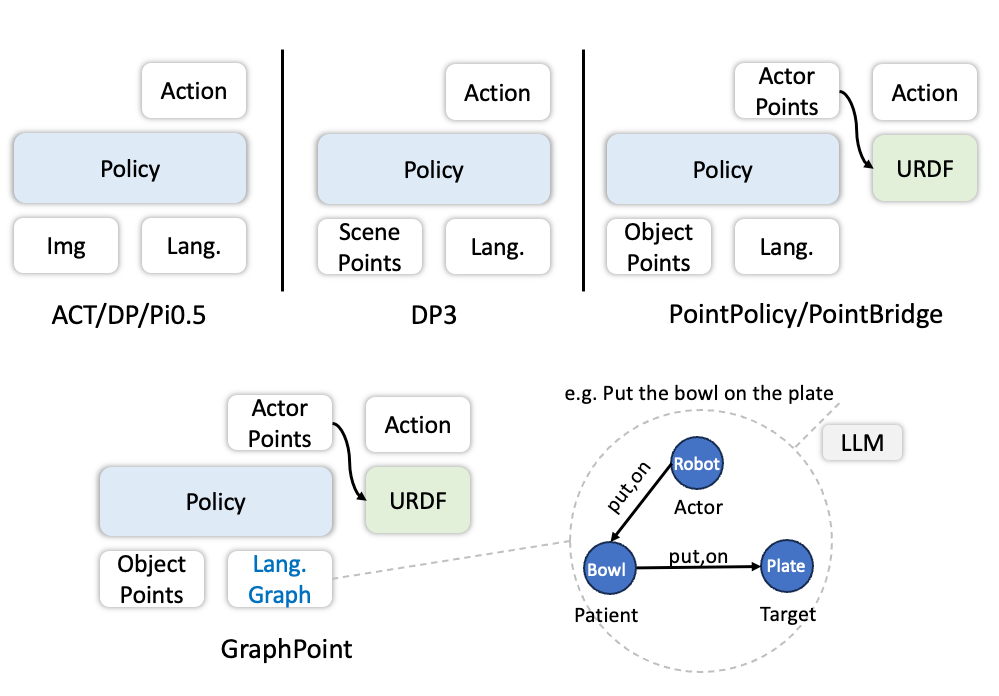
\includegraphics[width=\columnwidth]{fig/compare.png}
\caption{Policy representation interfaces.
GraphPoint organizes entity points into a language-conditioned role graph and converts predicted actor points into robot actions through gripper geometry.}
\label{fig:representation_comparison}
\end{figure}

To isolate these capabilities, we introduce CoMani, a LIBERO-based benchmark~\cite{liu2023libero} with suites for modifier, action-type, and sequential composition.
Matched initial scenes reduce visual task shortcuts, and atomic-only training separates skill acquisition from sequence execution.
Our contributions are:
\begin{itemize}
    \item CoMani, a benchmark addressing the need to distinguish composition of modifiers, action types, and atomic skills through controlled in-distribution (ID) and out-of-distribution (OOD) splits over 18 modifier tasks, 10 action tasks, and 6 sequences.
    \item GraphPoint, a framework coupling semantic entity graphs with task-conditioned point-trajectory control and progress-based subtask switching, validated through baseline comparisons and component ablations on CoMani.
\end{itemize}

\section{Related Work}

\textbf{Visual and point-based policies.}
ACT~\cite{zhao2023act} predicts action chunks, DP~\cite{chi2023dp} generates actions through conditional denoising, and $\pi_{0.5}$~\cite{physicalintelligence2025pi05} uses large-scale vision-language-action pretraining.
Geometric alternatives include DP3's sparse scene point clouds~\cite{ze2024dp3}, PointPolicy's semantic observation and action keypoints learned from human videos~\cite{haldar2025pp}, and PointBridge's unified points for synthetic-data training and sim-to-real transfer~\cite{haldar2026pb}.
GraphPoint organizes task-relevant points by semantic role and conditions their interaction on action types and modifiers.

\textbf{Object-centric and graph representations.}
GROOT~\cite{zhu2023groot} uses segmented object point clouds and segmentation correspondence for visual generalization.
GraphMimic~\cite{chen2025graphmimic} predicts object and visual-action graphs from videos to condition control.
Compose by Focus~\cite{qi2026compose} encodes task-relevant subgraphs and combines diffusion-based atomic skills with a vision-language planner.
Building on these established object-centric and graph-based approaches, GraphPoint couples actor/patient/target roles with explicit action/modifier conditioning and point-trajectory generation.

\textbf{Compositional generalization.}
CLIPort~\cite{shridhar2022cliport} combines semantic features with spatial action prediction; VIMA~\cite{jiang2023vima} evaluates multimodal prompting across four generalization levels.
CompoSuite~\cite{mendez2022composuite} holds out combinations of robots, objects, obstacles, and objectives, while LIBERO~\cite{liu2023libero} studies declarative and procedural transfer and CALVIN~\cite{mees2022calvin} evaluates language-conditioned task sequences.
CoMani isolates modifier composition, action-type composition, and three-step execution in LIBERO, using matched scenes to reduce visual task shortcuts and atomic-only training to test sequential reuse.

\section{Method}
\label{sec:method}

\subsection{Overview}
GraphPoint represents manipulation as interactions among 3D point entities and predicts future gripper points in the same geometric space.
As shown in Fig.~\ref{fig:framework}, language analysis, visual localization, and point tracking construct a task-conditioned entity graph, which a shared policy maps to a point trajectory and a subtask progress estimate.
For a multi-step instruction, the system instantiates this graph for each subtask and uses predicted progress to advance through the sequence.
The learned policy receives entity geometry and structured language conditions; color images are used by the perception front end.

\begin{figure*}[t]
\centering
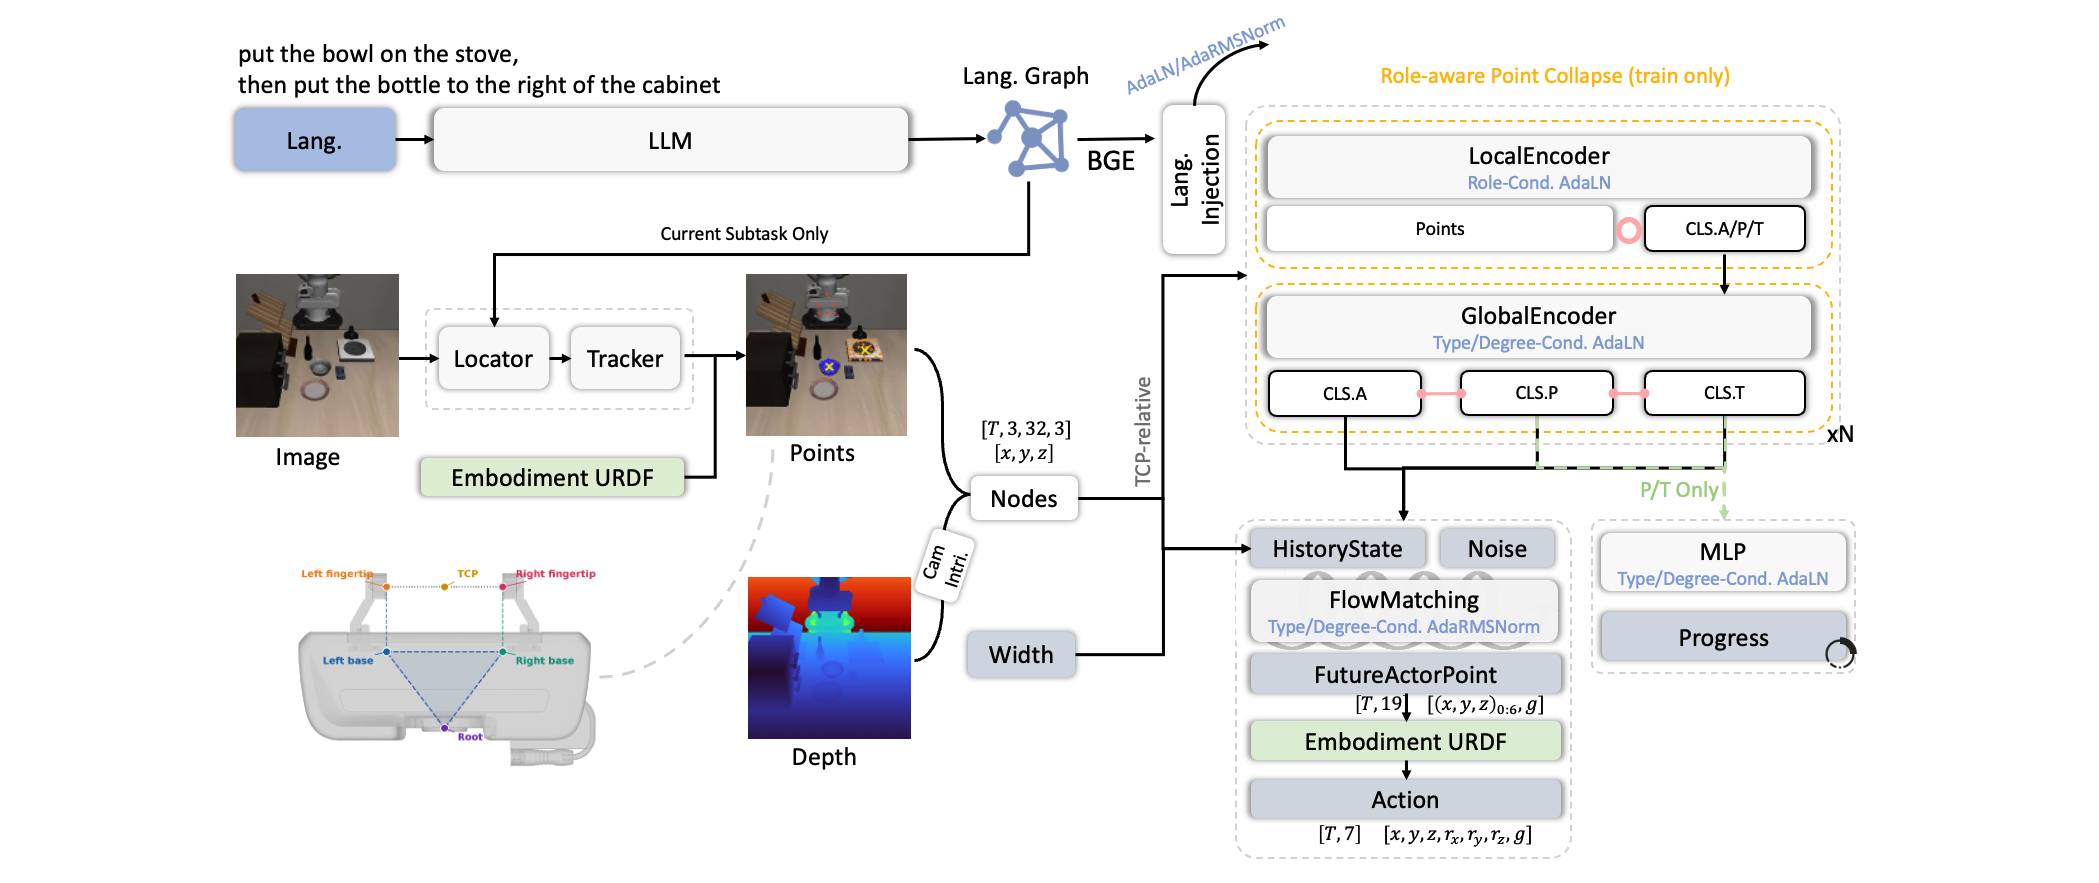
\includegraphics[width=\textwidth]{fig/main.png}
\caption{GraphPoint framework.
Language analysis identifies ordered subtasks and their semantic roles, while visual localization and tracking ground the relevant entities as 3D points.
The policy alternates local entity encoding with temporal graph attention, conditioned on roles, action types, and modifiers.
A flow decoder predicts future actor points and gripper commands, and a progress head supports subtask transitions.
Robot geometry converts predicted points into executable gripper poses.}
\label{fig:framework}
\end{figure*}
% Figure TODO: FutureActorPoint should have shape [H,19] for 6 XYZ points plus 1 gripper command, not [T,10].

\subsection{Task-to-Graph Construction}
\textbf{Semantic decomposition.}
A language model decomposes an instruction into ordered subtasks, each specified by an action type, a modifier, and entity roles.
The \emph{actor} $A$ denotes the gripper, the \emph{patient} $P$ denotes the manipulated object or part, and the \emph{target} $T$ denotes the reference entity.
For example, ``put the cheese to the right of the stove'' assigns cheese to $P$, stove to $T$, \emph{put} to the action type, and \emph{right} to the modifier.
Entity names guide visual grounding, whereas action types and modifiers are encoded separately using frozen BGE embeddings~\cite{xiao2024bge} and learned projections.
We denote their concatenation by the task condition $c$ and the learned embedding of role $r$ by $e_r$.
For readability, $c$ also denotes the version with separately normalized action and modifier embeddings used by the prediction heads.
Absent modifiers use a learned null embedding, and absent entities are masked.

\textbf{Grounded point entities.}
A pretrained vision-language locator identifies the requested objects or parts, and SAM~2~\cite{ravi2024sam2} produces masks from the localization prompts.
We sample 32 points per visual entity and track their image coordinates with TAPNext++~\cite{jung2026tapnextpp}.
Depth and camera intrinsics back-project these tracks into 3D.
The actor instead uses 6 keypoints computed from robot geometry and proprioception: the gripper root, TCP, 2 finger bases, and 2 fingertips.
We align all entities in camera coordinates and subtract the current TCP position from every point in the observation history and prediction horizon.
Thus, coordinates retain camera-axis orientation while sharing a translation origin at the current TCP.
This representation reduces dependence on absolute scene placement.
Actor points are padded with a validity mask, and coordinates are normalized using training-set quantiles.
The policy observes 10 frames, including the current frame.

\subsection{Role-Structured Entity Graph Encoder}
\textbf{Role-conditioned geometry and task-conditioned interaction.}
A shared point MLP embeds entity coordinates, with keypoint identity embeddings added for the actor.
Each entity at each observed time receives 4 learned CLS tokens to summarize its geometry.
The encoder alternates local encoding within each entity and global interaction among entity summaries:
\begin{equation}
\begin{aligned}
    (\widetilde C_r,F_r^{\ell+1})
       &=\operatorname{Local}_{\ell}(C_r^\ell,F_r^\ell;e_r),\\
    C^{\ell+1}
       &=\operatorname{Graph}_{\ell}(\{\widetilde C_r\}_{r\in\{A,P,T\}};c).
\end{aligned}
\label{eq:encoder}
\end{equation}
Here, $F_r$ and $C_r$ denote point features and CLS summaries, respectively, with observation-time indices omitted for clarity.
Local self-attention processes each entity and frame independently, conditioned on its role $e_r$.
Graph attention exchanges only CLS summaries across entities and observed times, conditioned on the action and modifier $c$.
Its connectivity follows the bidirectional chain $A\leftrightarrow P\leftrightarrow T$, with additional within-role temporal connections.
Direct actor--target attention is masked, so their interaction is mediated by the patient through successive layers.
This structure preserves separate entity summaries and encodes gripper--object and object--reference interactions.
Temporal rotary embeddings distinguish observation times.
After 8 layers, the current-time CLS summaries form memory $M_t$, incorporating both geometry and interaction history.

\textbf{Semantic injection.}
Both local and graph blocks contain attention and feed-forward sublayers, whose inputs are modulated through AdaLN:
\begin{equation}
    \operatorname{AdaLN}(h;q)
    =(1+\gamma(q))\odot\operatorname{LN}(h)+\beta(q).
\label{eq:adaln}
\end{equation}
The scale $\gamma$ and shift $\beta$ are learned functions of the condition, broadcast over tokens.
Local conditioning $q=e_r$ assigns roles to geometry; global conditioning $q=c$ distinguishes the instructed interaction, such as placing an object \emph{on} or to the \emph{right} of a target.

\textbf{Role-aware point collapse.}
During training, role-aware point collapse (RPC) independently collapses each patient or target point set with probability 0.05 to reduce dependence on detailed object shape.
For the patient, all points are replaced by the mean of the 4 points nearest to the TCP; for the target, they are replaced by the entity centroid.
This operation is applied consistently over the sampled temporal window, with anchors computed separately at each frame.
It preserves point counts and validity masks and leaves actor points and future action supervision unchanged.
The anchors retain the patient interaction region and target reference location while simplifying shape.

\subsection{Point-Trajectory Flow Policy}
We predict $H=10$ future steps, each containing 6 actor points and a scalar gripper command:
\begin{equation}
    Y=\{(X^A_{t+h},g_{t+h})\}_{h=1}^{H}.
\label{eq:point_trajectory}
\end{equation}
Here, $X^A_{t+h}$ contains actor coordinates relative to the current TCP, and $g_{t+h}$ is the open/close command.
Each step is represented by a 19-dimensional vector in point-wise $(x,y,z)$ order followed by the gripper command.
Representing actions as gripper points makes the predicted motion spatially comparable to the observed entities and encodes orientation through the arrangement of multiple points.

\textbf{Geometry- and language-conditioned decoding.}
A 6-layer Transformer models this trajectory with conditional flow matching~\cite{lipman2022flow}.
It embeds the observed actor history $U_t$ together with the noisy future trajectory $Z_\tau$ and predicts a velocity field:
\begin{equation}
    v_\theta=\operatorname{Decoder}_{\theta}(Z_\tau,U_t;M_t,c,\tau).
\label{eq:decoder}
\end{equation}
Each decoder layer uses self-attention to relate trajectory steps, cross-attention to retrieve entity geometry from $M_t$, and a feed-forward sublayer to update features.
Future tokens attend to both history and future, while history tokens cannot attend to future tokens.
Temporal rotary embeddings encode their relative times.
Action and modifier semantics enter every sublayer through AdaRMSNorm, following the scale-and-shift principle of Eq.~\eqref{eq:adaln}.
Separate mappings of the task condition $c$ and flow-time embedding are added to generate the scale, shift, and residual gate.
A final projection of the future tokens produces the point and gripper velocity predictions.

% Submit the benchmark figure early so it appears beside the benchmark introduction.
\begin{figure*}[!t]
    \centering
    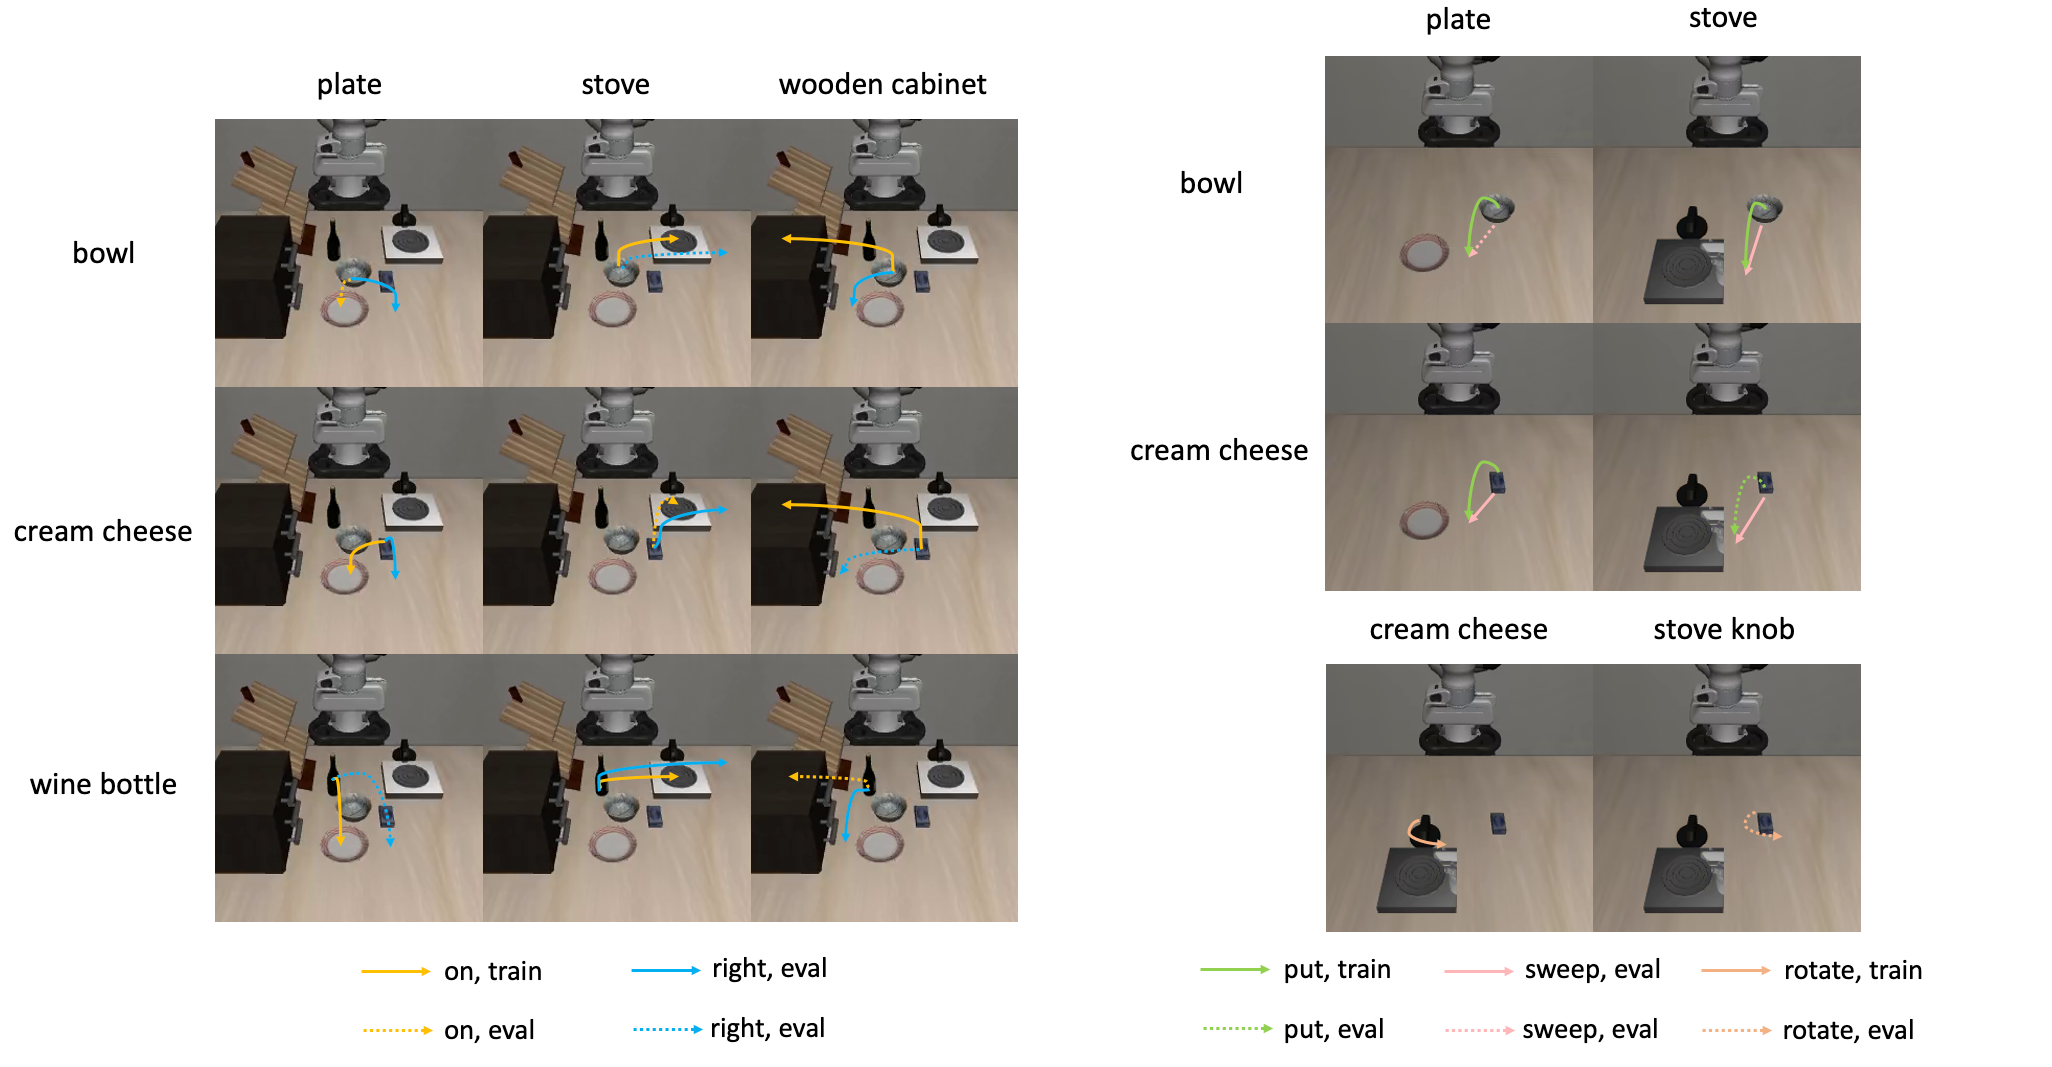
\includegraphics[width=\textwidth]{fig/benchmark.png}
    \caption{CoMani task construction and splits.
    Left: CoMani-Mod varies modifiers with a fixed put action.
    Center: CoMani-Act varies action types with a fixed right modifier.
    Right: CoMani-Seq composes atomic tasks from CoMani-Mod into 6 sequences of 3 steps, shown in 3 rows with execution proceeding from left to right.}
    \label{fig:benchmark}
\end{figure*}

\textbf{Training and execution.}
For a demonstrated trajectory $Y$ and Gaussian noise $\epsilon$, the flow objective is
\begin{equation}
\begin{aligned}
    Z_\tau&=(1-\tau)Y+\tau\epsilon,\\
    \mathcal L_{\mathrm{flow}}
       &=\mathbb E\!\left[\operatorname{MSE}(v_\theta,\epsilon-Y)\right],
\end{aligned}
\label{eq:flow}
\end{equation}
where the squared error is averaged over trajectory steps and output dimensions.
At inference, 10 Euler steps integrate from noise at $\tau=1$ to a trajectory at $\tau=0$.
After denormalization and restoring the TCP translation, we fit the robot's gripper keypoint template to each predicted point set using least-squares rigid alignment.
The template uses the observed gripper width, and the predicted gripper command is applied separately.
The recovered poses are transformed into the control frame and executed in a receding-horizon manner.

\subsection{Subtask Progress and Long-Horizon Composition}
The progress head estimates how far the active subtask has advanced from the current patient and target summaries:
\begin{equation}
    \hat{s}_t=\operatorname{Progress}_{\theta}(C_{t,P},C_{t,T};c).
\label{eq:progress}
\end{equation}
It uses a task-conditioned MLP with AdaLN and a sigmoid output, so the same geometry is evaluated under the active action and modifier.
The readout excludes direct actor summaries, although graph attention can propagate actor information into patient and target summaries.
Training targets increase linearly from 0 to 1 within each annotated subtask interval, and the complete objective is
\begin{equation}
    \mathcal{L}=\mathcal{L}_{\mathrm{flow}}+
    \operatorname{SmoothL1}(\hat{s}_t,s_t).
\end{equation}
At deployment, the planner advances when predicted progress exceeds a threshold for a consecutive window of policy calls.
We denote this learned transition rule as self-switching (SS).
Environment-based switching (ES) instead uses an environment-provided subtask completion signal to separate execution performance from learned transition timing.
On a transition, the system releases and lifts the gripper, selects the next subtask's entities and language conditions, and resets policy history.
The same atomic policy is reused throughout the sequence.

\section{CoMani Benchmark}
\label{sec:benchmark}

CoMani comprises 3 suites testing modifier, action-type, and sequential composition (Fig.~\ref{fig:benchmark}; Table~\ref{tab:comani_tasks}).
We generate 50 trajectories per atomic task using MimicGen~\cite{mandlekar2023mimicgen}.
Within each suite, initial scenes are matched wherever feasible to require instruction-dependent behavior and discourage fixed vision-to-action mappings.
We report success rates by split over 30 trials per atomic task and 10 per sequence.

\begin{figure*}[t]
    \centering
    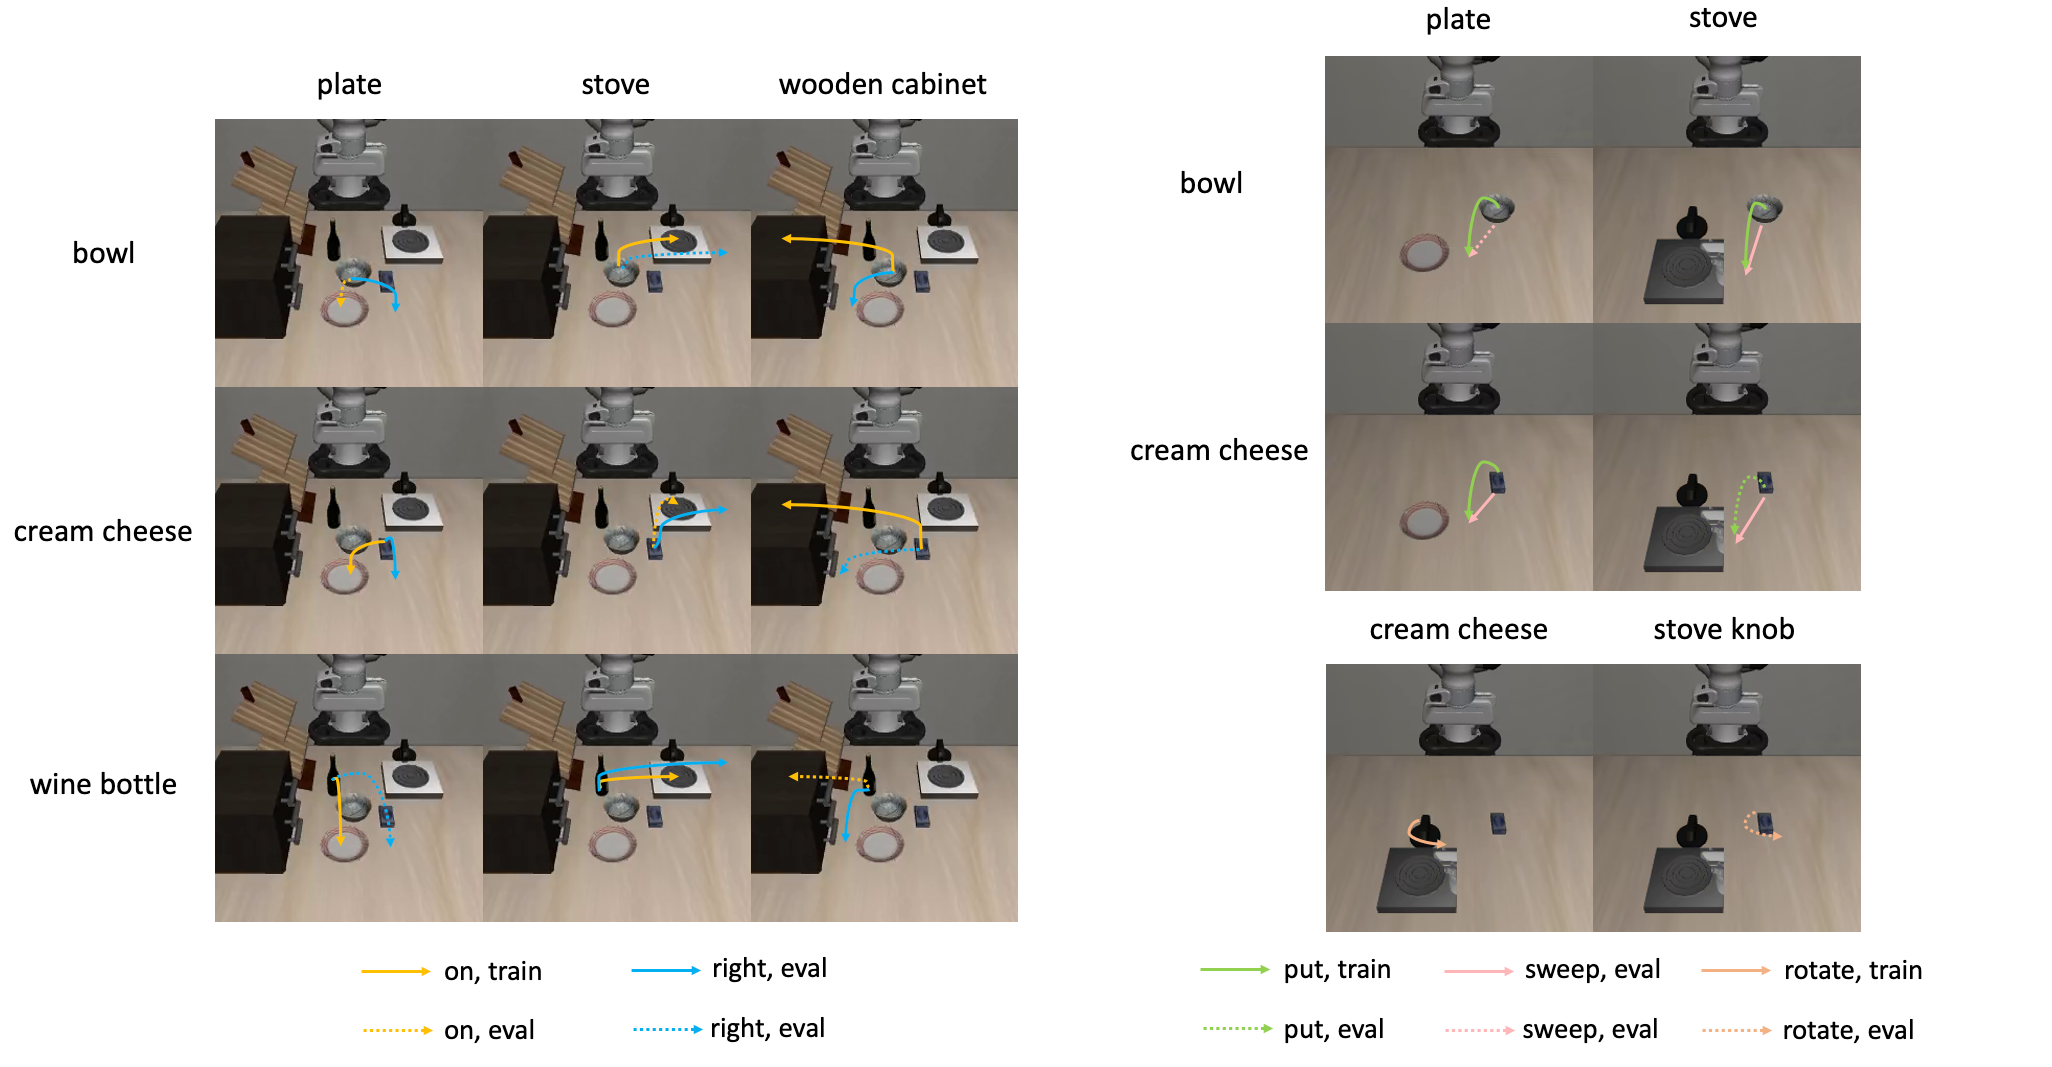
\includegraphics[width=\textwidth]{fig/benchmark.png}
    \caption{CoMani task construction and splits.
    Left: CoMani-Mod varies modifiers with a fixed put action.
    Center: CoMani-Act varies action types with a fixed right modifier.
    Right: CoMani-Seq composes atomic tasks from CoMani-Mod into six three-step sequences, shown in three rows with execution proceeding from left to right.}
    \label{fig:benchmark}
\end{figure*}

% Figure corrections pending: in the CoMani-Mod legend, dotted yellow means
% on/OOD and solid blue means right/ID.

\textbf{CoMani-Mod.} With pick-and-place (\emph{put}) fixed, this suite combines 3 objects, 3 targets, and 2 modifiers (\emph{on}/\emph{right of}) into 18 tasks: 12 in-distribution (ID) and 6 out-of-distribution (OOD).
Each OOD object--target pair appears in the ID split with the opposite modifier, isolating generalization to unseen combinations of familiar factors.
The ID/OOD comparison therefore tests whether a policy can apply the instructed relation to a familiar object--target pair beyond its demonstrated placement.

% Internal suite: 0902. Code ID-split IDs: 1,2,3,5,6,8,9,10,12,13,16,17.
% OOD IDs: 0,4,7,11,14,15. Held-out on: bowl/plate, cheese/stove,
% bottle/cabinet. Held-out right: bowl/stove, cheese/cabinet, bottle/plate.

\textbf{CoMani-Act.} With \emph{right} fixed, this suite varies \emph{put}, \emph{sweep}, and \emph{rotate} across 10 tasks: 7 ID and 3 OOD.
For put/sweep, each OOD object--target pair appears in the ID split with the other action; for rotation, the ID task uses the stove knob and the OOD task uses cream cheese.
These tests examine whether a policy can reuse an action with familiar entities in a new combination and transfer rotation across different manipulated entities.
Put/sweep pairs share initial states and final-position goals, so success measures goal attainment rather than interaction mode.

% Internal suite: 0904. Code ID-split IDs: 0,1,2,5,7,8,9. Code OOD-split IDs: 3,4,6.
% Rotation details: dataset term "right" means counterclockwise about world +Z
% viewed from above. Knob: joint position >= 0.5 rad. Cheese: reset-relative
% signed rotation >= 0.5 rad, with tilt <= 15 degrees.

\textbf{CoMani-Seq.} This suite tests whether policies learned from CoMani-Mod atomic demonstrations can execute 3-step instructions without sequence-level demonstrations.
It contains 6 sequences organized into 3 fixed-order pairs, each varying one modifier between \emph{on} and \emph{right of}, without permuting subtasks.
The 3 pairs contain 3 ID, 2 ID + 1 OOD, and 2/1 ID + 1/2 OOD atomic tasks, respectively (Fig.~\ref{fig:benchmark}, right).
The all-ID pair tests composition and transitions among familiar skills; the remaining pairs test whether execution also generalizes to held-out atomic combinations, with the last pair increasing the OOD count from 1 to 2 through a single modifier change.

% Internal suite: libero_custom_0906. Evaluation order: 0,1,2,3,4,5.
% Figure pair order: tasks 2/3 (3 ID), 0/1 (2 ID + 1 OOD), 4/5 (mixed).
% TODO: Specify shared-scene initialization, ordered subtask completion checks,
% whether earlier goals must remain satisfied, and the sequence time budget.
\begin{table*}[t]
\centering
\caption{CoMani task lists and ID/OOD splits.
In (c), ID/OOD gives atomic task counts; atomic IDs refer to (a), with OOD IDs underlined.}
% IMPORTANT: Paper IDs differ from code/evaluation IDs.
% Use expr/task_id_mapping.json when importing results; never match numeric IDs directly.
\label{tab:comani_tasks}
\footnotesize
\setlength{\tabcolsep}{2pt}
\renewcommand{\arraystretch}{1.08}
\begin{minipage}[t]{0.49\textwidth}
\centering
\textbf{(a) CoMani-Mod}\par\smallskip
% Match the height of the stacked Act and Seq tables on the right.
\renewcommand{\arraystretch}{1.532}
\begin{tabular*}{\linewidth}{@{\extracolsep{\fill}}r|p{6.35cm}|l}
\noalign{\hrule height 1pt}
ID & Task instruction & Split \\
\hline
0 & Put the bowl on the stove. & ID \\
1 & Put the bowl on the wooden cabinet. & ID \\
2 & Put the bowl to the right of the plate. & ID \\
3 & Put the bowl to the right of the wooden cabinet. & ID \\
4 & Put the cream cheese on the plate. & ID \\
5 & Put the cream cheese on the wooden cabinet. & ID \\
6 & Put the cream cheese to the right of the plate. & ID \\
7 & Put the cream cheese to the right of the stove. & ID \\
8 & Put the wine bottle on the plate. & ID \\
9 & Put the wine bottle on the stove. & ID \\
10 & Put the wine bottle to the right of the stove. & ID \\
11 & Put the wine bottle to the right of the wooden cabinet. & ID \\
\hline
12 & Put the bowl on the plate. & OOD \\
13 & Put the bowl to the right of the stove. & OOD \\
14 & Put the cream cheese on the stove. & OOD \\
15 & Put the cream cheese to the right of the wooden cabinet. & OOD \\
16 & Put the wine bottle on the wooden cabinet. & OOD \\
17 & Put the wine bottle to the right of the plate. & OOD \\
\noalign{\hrule height 1pt}
\end{tabular*}
\end{minipage}\hfill
\begin{minipage}[t]{0.49\textwidth}
\centering
\textbf{(b) CoMani-Act}\par\smallskip
\begin{tabular*}{\linewidth}{@{\extracolsep{\fill}}r|p{6.35cm}|l}
\noalign{\hrule height 1pt}
ID & Task instruction & Split \\
\hline
0 & Put the bowl to the right of the plate. & ID \\
1 & Put the bowl to the right of the stove. & ID \\
2 & Put the cream cheese to the right of the plate. & ID \\
3 & Rotate the stove knob right. & ID \\
4 & Sweep the bowl to the right of the stove. & ID \\
5 & Sweep the cream cheese to the right of the plate. & ID \\
6 & Sweep the cream cheese to the right of the stove. & ID \\
\hline
7 & Put the cream cheese to the right of the stove. & OOD \\
8 & Rotate the cream cheese right. & OOD \\
9 & Sweep the bowl to the right of the plate. & OOD \\
\noalign{\hrule height 1pt}
\end{tabular*}
\par\smallskip
\centering
\textbf{(c) CoMani-Seq}\par\smallskip
\begin{tabular*}{\linewidth}{@{\extracolsep{\fill}}r|l|p{4.7cm}|l}
\noalign{\hrule height 1pt}
ID & ID/OOD & Sequence & Atomic IDs \\
\hline
0 & 3/0 & Wine bottle on stove $\to$ cream cheese right of plate $\to$ bowl on wooden cabinet & $9\to6\to1$ \\
1 & 3/0 & Wine bottle right of stove $\to$ cream cheese right of plate $\to$ bowl on wooden cabinet & $10\to6\to1$ \\
\hline
2 & 2/1 & Wine bottle on stove $\to$ bowl on plate $\to$ cream cheese on wooden cabinet & $9\to\underline{12}\to5$ \\
3 & 2/1 & Wine bottle right of stove $\to$ bowl on plate $\to$ cream cheese on wooden cabinet & $10\to\underline{12}\to5$ \\
\hline
4 & 2/1 & Cream cheese right of plate $\to$ bowl on stove $\to$ wine bottle on wooden cabinet & $6\to0\to\underline{16}$ \\
5 & 1/2 & Cream cheese right of plate $\to$ bowl right of stove $\to$ wine bottle on wooden cabinet & $6\to\underline{13}\to\underline{16}$ \\
\noalign{\hrule height 1pt}
\end{tabular*}
\end{minipage}
\end{table*}

\section{Experiments}

\begin{table*}[!t]
\centering
\caption{CoMani-Mod success rates.
Task IDs follow Table~\ref{tab:comani_tasks}.}
\label{tab:modifier_comparison}
\fontsize{7}{8.4}\selectfont
\setlength{\tabcolsep}{1.5pt}
\renewcommand{\arraystretch}{1.15}
\def\resultcolwidth{\dimexpr(\textwidth-2pt-1.7cm-42\tabcolsep-3\arrayrulewidth)/20\relax}
\begin{tabular}{p{1.7cm}|*{2}{>{\centering\arraybackslash}p{\resultcolwidth}}|*{12}{>{\centering\arraybackslash}p{\resultcolwidth}}|*{6}{>{\centering\arraybackslash}p{\resultcolwidth}}}
\noalign{\hrule height 1pt}
\multirow[c]{2}{*}{Method} & \multicolumn{2}{c|}{Mean SR} & \multicolumn{12}{c|}{ID SR} & \multicolumn{6}{c}{OOD SR} \\
\cline{2-21}
 & ID & OOD & 0 & 1 & 2 & 3 & 4 & 5 & 6 & 7 & 8 & 9 & 10 & 11 & 12 & 13 & 14 & 15 & 16 & 17 \\
\hline
% PointBridge sources: server 9996, point_bridge_points_custom0902-step_30000; ID libero_custom_0902-0912-025321-346811/result.json (103/360); OOD libero_custom_0902-0912-025322-202611/result.json (6/180). Verified against per-episode records and mapped through expr/task_id_mapping.json.
PointBridge & 28.6 & 3.3 & 0.0 & 36.7 & 60.0 & \textbf{100.0} & 0.0 & 0.0 & 83.3 & 63.3 & 0.0 & 0.0 & 0.0 & 0.0 & 20.0 & 0.0 & 0.0 & 0.0 & 0.0 & 0.0 \\
PointPolicy & 21.4 & 15.0 & 3.3 & 36.7 & 66.7 & 50.0 & 0.0 & 0.0 & 16.7 & 0.0 & 23.3 & 0.0 & 13.3 & 46.7 & 10.0 & 0.0 & 0.0 & 6.7 & 0.0 & 73.3 \\
DP3 & 73.6 & 57.2 & 73.3 & \textbf{100.0} & \textbf{100.0} & \textbf{100.0} & 53.3 & \textbf{100.0} & 0.0 & 80.0 & 80.0 & 86.7 & 26.7 & 83.3 & 86.7 & \textbf{63.3} & 60.0 & \textbf{93.3} & 16.7 & 23.3 \\
ACT & 20.0 & 7.2 & 33.3 & 20.0 & 6.7 & 23.3 & 13.3 & 56.7 & 10.0 & 3.3 & 63.3 & 0.0 & 0.0 & 10.0 & 30.0 & 0.0 & 0.0 & 13.3 & 0.0 & 0.0 \\
DP & 40.0 & 10.0 & 43.3 & 36.7 & 16.7 & 26.7 & 50.0 & 66.7 & 20.0 & 33.3 & 80.0 & 16.7 & 36.7 & 53.3 & 30.0 & 0.0 & 0.0 & 30.0 & 0.0 & 0.0 \\
$\pi_{0.5}$ & 91.1 & 48.3 & \textbf{100.0} & \textbf{100.0} & 56.7 & \textbf{100.0} & 73.3 & \textbf{100.0} & 96.7 & \textbf{83.3} & \textbf{100.0} & \textbf{100.0} & 83.3 & \textbf{100.0} & 80.0 & 33.3 & 6.7 & 80.0 & 6.7 & \textbf{83.3} \\
\hline
GraphPoint & \textbf{96.4} & \textbf{75.6} & \textbf{100.0} & \textbf{100.0} & \textbf{100.0} & 86.7 & \textbf{93.3} & \textbf{100.0} & \textbf{100.0} & 80.0 & \textbf{100.0} & \textbf{100.0} & \textbf{96.7} & \textbf{100.0} & \textbf{100.0} & \textbf{63.3} & \textbf{73.3} & 76.7 & \textbf{73.3} & 66.7 \\
\noalign{\hrule height 1pt}
\end{tabular}
\end{table*}

\begin{table*}[!t]
\centering
\caption{CoMani-Act action-consistent success rates (ACSR).
Task IDs follow Table~\ref{tab:comani_tasks}.}
\label{tab:action_comparison}
\fontsize{7}{8.4}\selectfont
\setlength{\tabcolsep}{1.5pt}
\renewcommand{\arraystretch}{1.15}
\def\resultcolwidth{\dimexpr(\textwidth-2pt-1.7cm-26\tabcolsep-3\arrayrulewidth)/12\relax}
\begin{tabular}{p{1.7cm}|*{2}{>{\centering\arraybackslash}p{\resultcolwidth}}|*{7}{>{\centering\arraybackslash}p{\resultcolwidth}}|*{3}{>{\centering\arraybackslash}p{\resultcolwidth}}}
\noalign{\hrule height 1pt}
\multirow[c]{2}{*}{Method} & \multicolumn{2}{c|}{Mean ACSR} & \multicolumn{7}{c|}{ID ACSR} & \multicolumn{3}{c}{OOD ACSR} \\
\cline{2-13}
 & ID & OOD & 0 & 1 & 2 & 3 & 4 & 5 & 6 & 7 & 8 & 9 \\
\hline
PointPolicy & 80.5 & 4.4 & \textbf{100.0} & 73.3 & 23.3 & \textbf{100.0} & \textbf{100.0} & 76.7 & 90.0 & 13.3 & 0.0 & 0.0 \\
DP3 & 83.3 & 60.0 & 80.0 & 93.3 & \textbf{96.7} & \textbf{100.0} & \textbf{100.0} & 86.7 & 26.7 & \textbf{80.0} & 0.0 & \textbf{100.0} \\
$\pi_{0.5}$ &  &  &  &  &  &  &  &  &  &  &  &  \\
\hline
GraphPoint & \textbf{90.5} & \textbf{64.4} & 50.0 & \textbf{100.0} & 83.3 & \textbf{100.0} & \textbf{100.0} & \textbf{100.0} & \textbf{100.0} & 26.7 & \textbf{76.7} & 90.0 \\
\noalign{\hrule height 1pt}
\end{tabular}
\end{table*}

% Defer the sequence and following ablation tables by one page.
\afterpage{\afterpage{
\begin{table*}[!t]
\centering
\caption{CoMani-Seq success rate (SR) and progress rate (PR).
Environment-based switching (ES) uses goal signals; self-switching (SS) uses predicted progress.
Mean groups by OOD count; task IDs follow Table~\ref{tab:comani_tasks}.}
\label{tab:sequence_comparison}
\fontsize{7}{8.4}\selectfont
\setlength{\tabcolsep}{1.5pt}
\renewcommand{\arraystretch}{1.15}
\def\resultcolwidth{\dimexpr(\textwidth-2pt-4.3cm-44\tabcolsep-11\arrayrulewidth)/20\relax}
\begin{tabular}{p{3.3cm}|>{\centering\arraybackslash}p{1.0cm}|*{9}{*{2}{>{\centering\arraybackslash}p{\resultcolwidth}}|}*{2}{>{\centering\arraybackslash}p{\resultcolwidth}}}
\noalign{\hrule height 1pt}
\multirow[c]{3}{*}{Method} & \multirow[c]{3}{*}{Switch} & \multicolumn{8}{c|}{Mean} & \multicolumn{4}{c|}{3 ID} & \multicolumn{4}{c|}{2 ID + 1 OOD} & \multicolumn{4}{c}{2/1 ID + 1/2 OOD} \\
\cline{3-22}
 & & \multicolumn{2}{c|}{All} & \multicolumn{2}{c|}{0 OOD} & \multicolumn{2}{c|}{1 OOD} & \multicolumn{2}{c|}{2 OOD} & \multicolumn{2}{c|}{0} & \multicolumn{2}{c|}{1} & \multicolumn{2}{c|}{2} & \multicolumn{2}{c|}{3} & \multicolumn{2}{c|}{4} & \multicolumn{2}{c}{5} \\
\cline{3-22}
 & & SR & PR & SR & PR & SR & PR & SR & PR & SR & PR & SR & PR & SR & PR & SR & PR & SR & PR & SR & PR \\
\hline
PointPolicy & ES & 0.0 & 0.0 & 0.0 & 0.0 & 0.0 & 0.0 & 0.0 & 0.0 & 0.0 & 0.0 & 0.0 & 0.0 & 0.0 & 0.0 & 0.0 & 0.0 & 0.0 & 0.0 & 0.0 & 0.0 \\
DP3 & ES & 0.0 & 11.1 & 0.0 & 16.7 & 0.0 & 11.1 & 0.0 & 0.0 & 0.0 & 26.7 & 0.0 & 6.7 & 0.0 & 30.0 & 0.0 & 3.3 & 0.0 & 0.0 & 0.0 & 0.0 \\
$\pi_{0.5}$ & ES & 0.0 & 25.0 & 0.0 & 28.3 & 0.0 & 26.7 & 0.0 & 13.3 & 0.0 & 33.3 & 0.0 & 23.3 & 0.0 & 33.3 & 0.0 & 33.3 & 0.0 & 13.3 & 0.0 & 13.3 \\
\hline
GraphPoint & ES & 51.7 & 79.4 & 75.0 & 95.0 & 50.0 & 81.1 & 10.0 & 43.3 & 60.0 & 90.0 & 90.0 & 100.0 & 30.0 & 76.7 & 30.0 & 70.0 & 90.0 & 96.7 & 10.0 & 43.3 \\
GraphPoint & SS & 38.3 & 78.3 & 65.0 & 90.0 & 26.7 & 77.8 & 20.0 & 56.7 & 90.0 & 96.7 & 40.0 & 83.3 & 20.0 & 76.7 & 10.0 & 73.3 & 50.0 & 83.3 & 20.0 & 56.7 \\
\noalign{\hrule height 1pt}
\end{tabular}
\end{table*}
\begin{table*}[!t]
\centering
\caption{CoMani-Mod ablation success rates.
Task IDs follow Table~\ref{tab:comani_tasks}.}
\label{tab:modifier_ablation}
\fontsize{7}{8.4}\selectfont
\setlength{\tabcolsep}{1.5pt}
\renewcommand{\arraystretch}{1.15}
\def\resultcolwidth{\dimexpr(\textwidth-2pt-3.0cm-42\tabcolsep-3\arrayrulewidth)/20\relax}
\begin{tabular}{p{3.0cm}|*{2}{>{\centering\arraybackslash}p{\resultcolwidth}}|*{12}{>{\centering\arraybackslash}p{\resultcolwidth}}|*{6}{>{\centering\arraybackslash}p{\resultcolwidth}}}
\noalign{\hrule height 1pt}
\multirow[c]{2}{*}{Variant} & \multicolumn{2}{c|}{Mean SR} & \multicolumn{12}{c|}{ID SR} & \multicolumn{6}{c}{OOD SR} \\
\cline{2-21}
 & ID & OOD & 0 & 1 & 2 & 3 & 4 & 5 & 6 & 7 & 8 & 9 & 10 & 11 & 12 & 13 & 14 & 15 & 16 & 17 \\
\hline
w/o RPC & 90.6 & 44.4 & \textbf{100.0} & 96.7 & \textbf{100.0} & \textbf{100.0} & 66.7 & 96.7 & 96.7 & 83.3 & 93.3 & \textbf{100.0} & 70.0 & 83.3 & 20.0 & \textbf{90.0} & \textbf{80.0} & 6.7 & 10.0 & 60.0 \\
Full connectivity & 95.3 & 63.9 & 96.7 & 96.7 & \textbf{100.0} & \textbf{100.0} & \textbf{100.0} & 83.3 & \textbf{100.0} & \textbf{86.7} & \textbf{100.0} & \textbf{100.0} & 80.0 & \textbf{100.0} & 66.7 & 86.7 & 70.0 & 50.0 & 36.7 & \textbf{73.3} \\
Merged entity point set & 82.8 & 27.8 & 93.3 & 96.7 & \textbf{100.0} & \textbf{100.0} & 93.3 & 26.7 & 83.3 & 56.7 & \textbf{100.0} & 96.7 & 50.0 & 96.7 & 60.0 & 0.0 & 36.7 & 3.3 & 3.3 & 63.3 \\
Absolute point coordinates & 92.5 & 25.0 & 90.0 & \textbf{100.0} & \textbf{100.0} & 96.7 & 86.7 & \textbf{100.0} & 96.7 & 46.7 & \textbf{100.0} & \textbf{100.0} & 93.3 & \textbf{100.0} & 3.3 & 63.3 & 3.3 & 6.7 & 6.7 & 66.7 \\
Delta-action output & 95.0 & 73.3 & 96.7 & \textbf{100.0} & \textbf{100.0} & \textbf{100.0} & \textbf{100.0} & 96.7 & 80.0 & \textbf{86.7} & \textbf{100.0} & \textbf{100.0} & 80.0 & \textbf{100.0} & 96.7 & 86.7 & 76.7 & \textbf{76.7} & 50.0 & 53.3 \\
\hline
GraphPoint & \textbf{96.4} & \textbf{75.6} & \textbf{100.0} & \textbf{100.0} & \textbf{100.0} & 86.7 & 93.3 & \textbf{100.0} & \textbf{100.0} & 80.0 & \textbf{100.0} & \textbf{100.0} & \textbf{96.7} & \textbf{100.0} & \textbf{100.0} & 63.3 & 73.3 & \textbf{76.7} & \textbf{73.3} & 66.7 \\
\noalign{\hrule height 1pt}
\end{tabular}
\end{table*}
}}

\begin{figure*}[!t]
\centering
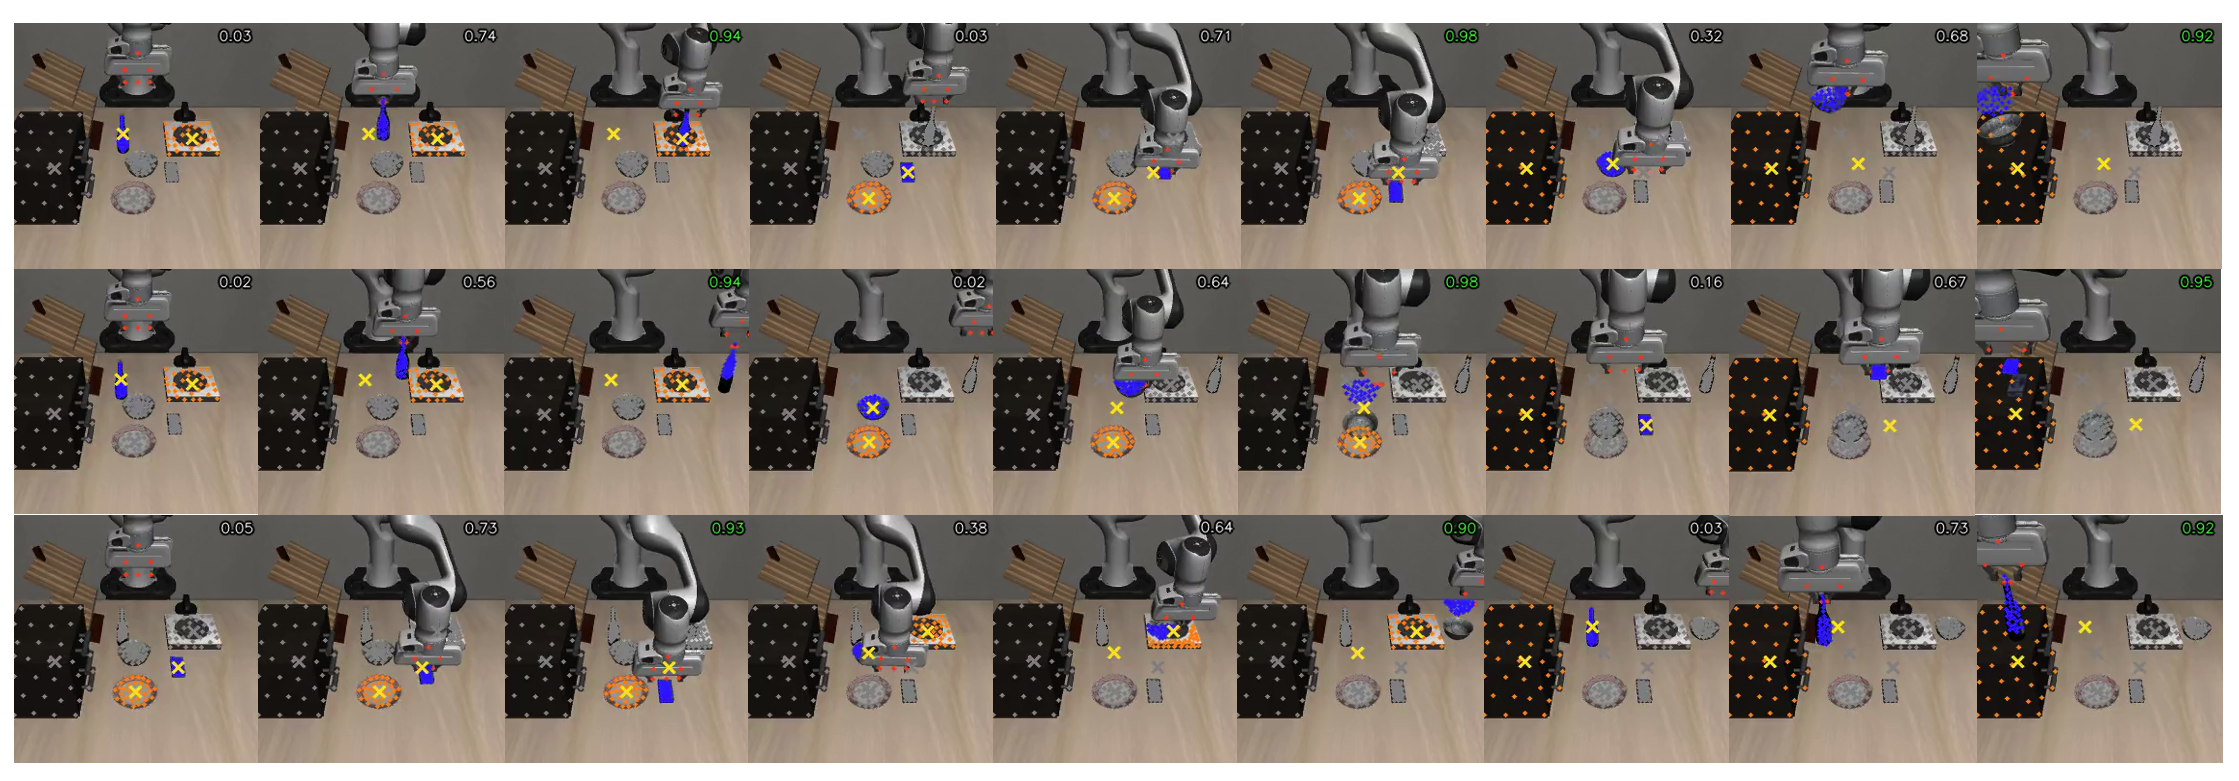
\includegraphics[width=\textwidth]{fig/vis.png}
\caption{Successful GraphPoint SS rollouts on CoMani-Seq.
Rows show sequences containing 0, 1, and 2 OOD subtasks, respectively, from top to bottom.
Each row proceeds from left to right, with 3 frames per subtask showing its start, execution, and completion.
Upper-right values show predicted subtask progress.
Apparent point-tracking mismatches are visualization artifacts, not actual tracking failures.}
\label{fig:sequence_rollouts}
\end{figure*}



\subsection{Experimental Setup}
\textbf{Baselines and adaptation.}
We compare GraphPoint with ACT~\cite{zhao2023act}, DP~\cite{chi2023dp}, DP3~\cite{ze2024dp3}, PointPolicy~\cite{haldar2025pp}, PointBridge~\cite{haldar2026pb}, and $\pi_{0.5}$~\cite{physicalintelligence2025pi05}.
ACT and DP use color images and robot state; DP3 uses scene point clouds and state. PointPolicy and PointBridge use LIBERO entity points and gripper-point supervision.
We adapt ACT, DP, DP3, and PointPolicy to multi-task instructions using frozen BGE embeddings of the full instruction, without role/action/modifier decomposition.
ACT projects this embedding into an additional Transformer encoder token; PointPolicy appends a projected language token to its point-token sequence.
DP and DP3 combine language and observation features through their existing FiLM conditioning paths.
PointBridge retains its native language-token pathway: frozen MiniLM sentence embeddings pass through a learned MLP and precede observation tokens in the causal Transformer.
$\pi_{0.5}$ retains its native image--text prefix conditioning and is fine-tuned with LoRA, without an added BGE encoder.
For CoMani-Seq, atomic policies are reused without sequence-level training, receiving the active subtask instruction under a shared ES protocol; GraphPoint is also evaluated with SS.

\textbf{Training and evaluation.}
All models are trained or fine-tuned on the first 10 demonstrations of each ID task for 30,000 steps with batch size 64 and AdamW; OOD tasks are excluded from training.
We evaluate at 20\,Hz over 30 trials per task on CoMani-Mod and CoMani-Act, and 10 trials per sequence on CoMani-Seq, using the splits in Sec.~\ref{sec:benchmark}.
Sequence rollouts allow 1,500 action steps after 30 settling steps and share initial-state indices across methods.
We use the suite-specific metrics defined in Sec.~\ref{sec:benchmark}: SR for CoMani-Mod, ACSR for CoMani-Act, and SR/PR for CoMani-Seq.
Tables report task means and ID/OOD aggregates, with unfinished evaluations left blank.

We evaluate modifier and action composition, sequential skill reuse, and component contributions.
% IMPORTANT: Map code IDs through expr/task_id_mapping.json before entering results.
% Existing numeric result columns retain their original task correspondence.
% Sources: expr/1.csv (Modifier comparison and ablations), expr/2.csv (Action).
% PI05 CoMani-Mod source: openpi/data/libero/pi05_custom0902_step29999/{id,ood}, 30 trials/task.
% Aggregate rates are copied from CSV SR-ID/SR-OOD, avoiding re-averaging rounded task percentages.
% Pending baseline cells must be filled from completed evaluations, not inferred from expected rankings.

\subsection{Can GraphPoint Generalize Across Modifiers?}
Table~\ref{tab:modifier_comparison} shows 96.4\% ID and 75.6\% OOD success for GraphPoint, exceeding the strongest baselines, $\pi_{0.5}$ on ID and DP3 on OOD, by 5.3 and 18.3 percentage points.
ACT, DP, PointPolicy, and PointBridge have low ID success, so their OOD results reflect limitations in both task acquisition and generalization.
GraphPoint achieves at least 63.3\% on every OOD task, compared with DP3's 16.7--93.3\% range.
For wine-bottle placement on the cabinet, it reaches 73.3\% versus 16.7\%; however, DP3 leads on placing cream cheese right of the cabinet (93.3\% versus 76.7\%).
These results support broader held-out relation coverage, while leaving an ID--OOD gap.

\subsection{Can GraphPoint Generalize Across Actions?}
Table~\ref{tab:action_comparison} evaluates action composition on CoMani-Act; $\pi_{0.5}$ results remain pending. PointPolicy reaches 80.5\% ID and 4.4\% OOD ACSR.
GraphPoint reaches 90.5\% ID and 64.4\% OOD ACSR, compared with 83.3\% and 60.0\% for DP3.
The modest average OOD advantage masks substantial differences across held-out tasks.
GraphPoint transfers rotation from the stove knob to cream cheese with 76.7\% ACSR, while DP3 obtains 0\%.
GraphPoint trails DP3 on putting cream cheese to the right of the stove, with 26.7\% versus 80.0\%, and on sweeping the bowl to the right of the plate, with 90.0\% versus 100.0\%.
Thus, these results support cross-entity rotation transfer but do not establish a uniform advantage across action combinations.
% PointPolicy Act sources: point_policy_custom0904-step_30000/libero_custom_0904-0913-131340-809426 and libero_custom_0904-0913-131421-638036; 300 unique completed episodes; author action review excludes 13 terminal successes for code task 3 (paper task 7), leaving 4/30. Raw final_goals records are preserved. Paper order: 0,1,2,5,7,8,9,3,4,6.
% The author confirmed that the reported CoMani-Act rates include action-process checks.

\subsection{Can GraphPoint Compose Atomic Skills?}
Table~\ref{tab:sequence_comparison} evaluates atomic policies on six three-step sequences without sequence-level training.
GraphPoint achieves 51.7\% SR and 79.4\% PR with ES, versus 38.3\% and 78.3\% with SS using patient/target progress summaries.
The 13.33-point SR drop despite a 1.11-point PR decrease shows that similar partial progress does not guarantee full completion.
With ES, PointPolicy, DP3, and $\pi_{0.5}$ all obtain 0\% SR, with PR of 0.0\%, 11.1\%, and 25.0\%, respectively.
GraphPoint's ES success decreases from 75.0\% with no OOD subtasks to 50.0\% with one and 10.0\% with two.
In the final task pair, changing only bowl-on-stove to the OOD bowl-right-of-stove subtask reduces SR from 90.0\% to 10.0\%, illustrating how atomic generalization limits sequence completion.
Fig.~\ref{fig:sequence_rollouts} shows successful SS executions across all three OOD counts and their entity/progress transitions.

% Including actor summaries (A+P+T) yields 41.67\% SR and 74.44\% PR under self-switching, compared with 38.33\% and 78.33\% for P+T. The mixed changes do not establish a consistent advantage for either progress-head input on these 60 trials.
% Seq paper IDs 0,1,2,3,4,5 map to code IDs 2,3,0,1,4,5.
% Use expr/task_id_mapping.json when entering results; display SR and PR as percentages to 1 decimal.
% Completed Seq sources: DP3 oracle 0913-045046-444735; GP oracle 0913-032319-902357; GP predicted 0913-033203-484464.
% PointPolicy Seq source: point_policy_custom0902-step_30000/libero_custom_0906-oracle-0913-093609-073005/result.json (60/60 episodes; verified against dualgpu0/1 partitions and per-episode records).
% PI05 Seq source: custom0902_id10ep-29999/libero_custom_0906-oracle-0913-085835-851951/result.json (60/60 episodes).
% A+P+T Seq source: allprogress predicted 0913-045808-238820 (60/60 episodes).
% Hidden row (preserved values): GraphPoint (A+P+T) & SS & 41.7 & 74.4 & 85.0 & 93.3 & 16.7 & 64.4 & 30.0 & 66.7 & 90.0 & 100.0 & 80.0 & 86.7 & 20.0 & 63.3 & 10.0 & 63.3 & 20.0 & 66.7 & 30.0 & 66.7 \\
% SR uses result.success_rate; PR uses result.progress_rate (not server_success_rate).

\subsection{Which Components Matter?}
Table~\ref{tab:modifier_ablation} examines GraphPoint variants on CoMani-Mod.
We remove RPC, replace chain attention with full connectivity, merge the entity graph into a single point set, use absolute point coordinates, or predict Cartesian delta actions instead of point trajectories.

\textbf{Geometry and graph structure.}
Removing RPC reduces OOD success by 31.1 percentage points, compared with a 5.8-point ID decrease, consistent with its intended role in reducing dependence on detailed training geometry.
Full graph connectivity retains 95.3\% ID success but lowers OOD success to 63.9\%, supporting patient-mediated interaction as a useful inductive bias.
Merging all entity points yields 27.8\% OOD success despite retaining 12 summary tokens in total.
This variant jointly removes role embeddings, separate local entity groups, and chain connectivity, and reads shared summaries for progress; it therefore tests the structured encoder as a whole rather than any single component.

\textbf{Coordinate and output representations.}
Using absolute point coordinates lowers OOD success to 25.0\% while retaining 92.5\% ID success, indicating that relative geometry is particularly useful for held-out combinations.
Replacing point trajectories with Cartesian delta actions gives 95.0\% ID and 73.3\% OOD success, close to the full model.
The observed gains are therefore more pronounced for relative coordinates, geometric augmentation, and role structure than for point output alone.
These comparisons describe the reported checkpoint evaluations; repeated-training estimates are needed to assess the reliability of small differences.

\FloatBarrier
\section{Conclusion}
We introduced CoMani to isolate modifier, action-type, and sequential composition, and GraphPoint to connect semantic entity graphs with point-trajectory control.
Results support role-structured interaction, TCP-relative geometry, and role-aware augmentation, while self-switching remains challenging.
Evaluation is limited to simulation, 3-step sequences, and a small set of entities and modifiers.
Occlusion can disrupt localization and tracking; upstream language parsing, localization, and segmentation add processing overhead and can propagate errors to control.
Despite focusing on task-relevant entities, the system lacks explicit obstacle avoidance for surrounding objects.
Future work will improve perception robustness, front-end efficiency, and obstacle-aware control.
The point-input, point-output interface also provides a common geometric representation for exploring transfer from simulation and human videos, and across robot embodiments; these capabilities remain to be evaluated.


\bibliographystyle{IEEEtranBST/IEEEtran}
\bibliography{IEEEtranBST/ref}

\end{document}
